\documentclass[border=4pt]{standalone}
% Preámbulo común de las figuras. Cada figura es un documento standalone
% que se compila a SVG con scripts/build_figures.sh
\usepackage[utf8]{inputenc}
\usepackage{amsmath}
\usepackage{tikz}
\usepackage[american, siunitx]{circuitikz}
\usetikzlibrary{arrows.meta,calc,decorations.pathmorphing,patterns}
\tikzset{
  >={Stealth[length=2.2mm]},
  eje/.style={->, thin},
  hilo/.style={thick},
}
% Paleta común: tonos medios legibles sobre fondo claro
\definecolor{azul}{RGB}{31,94,168}
\definecolor{rojo}{RGB}{192,57,43}
\definecolor{verde}{RGB}{39,128,73}
\definecolor{naranja}{RGB}{211,120,30}
\definecolor{morado}{RGB}{125,60,152}

\begin{document}
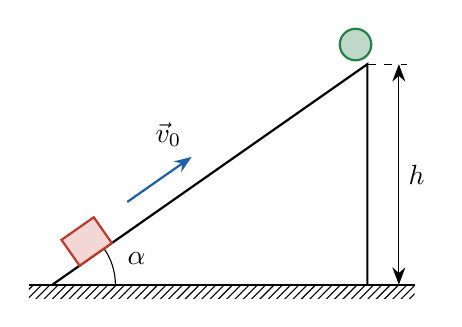
\begin{tikzpicture}[scale=1.0]
  % rampa de 35 grados: base 4.0, altura 2.8
  \fill[pattern=north east lines] (-0.3,-0.18) rectangle (4.6,0);
  \draw[thick] (-0.3,0) -- (4.6,0);
  \draw[thick] (0,0) -- (4,2.8) -- (4,0);
  \draw (0.8,0) arc (0:35:0.8); \node at (17.5:1.12) {$\alpha$};
  \begin{scope}[shift={(0.55,0.385)}, rotate=35]
    \filldraw[draw=rojo, fill=rojo!20, thick] (-0.25,0) rectangle (0.25,0.4);
  \end{scope}
  \draw[->, thick, azul] (0.95,1.05) -- ++(35:1.0) node[above left, text=black]{$\vec v_0$};
  \filldraw[draw=verde, fill=verde!30, thick] (3.85,3.05) circle (0.2);
  \draw[<->, thin] (4.4,0) -- node[right]{$h$} (4.4,2.8);
  \draw[dashed, thin] (4,2.8) -- (4.5,2.8);
\end{tikzpicture}
\end{document}
